\documentclass{article}

\usepackage{algorithm2e}
\usepackage{amsmath}
\usepackage{amssymb}
\usepackage{amsthm}
\usepackage{authblk}
\usepackage[english]{babel}
\usepackage{blkarray}
\usepackage[font=small]{caption}
\usepackage{cite}
\usepackage{graphicx}

\setlength{\thickmuskip}{2mu plus 3mu minus 1mu}
\setlength{\medmuskip}{1mu plus 2mu minus 1mu}

\SetKwComment{Comment}{$\triangleright$\ }{}

% ---- Author affiliations ---- %

\renewcommand\Affilfont{\itshape\small}

% ---- Propositions, lemmas, defintions... ---- %

%\newtheorem{algorithm}{Algorithm}
\newtheorem{corollary}{Corollary}
\newtheorem{definition}{Definition}
%\newtheorem{example}{Example}
\newtheorem{lemma}{Lemma}
\newtheorem{proposition}{Proposition}
%\newtheorem{remark}{Remark}


% ---- Special environments (examples and remarks) ---- %

\newcounter{examplecounter}
\newenvironment{example}
{\small\vspace{0.5\baselineskip}
  \refstepcounter{examplecounter}%
  \noindent\textbf{Example \arabic{examplecounter}.}%
}{\vspace{-0.2\baselineskip}\begin{center}%
  $\star$\end{center}\vspace{0.5\baselineskip}}

\newcounter{remarkcounter}
\newenvironment{remark}
{\small\it\vspace{0.5\baselineskip}
  \refstepcounter{remarkcounter}%
  \noindent\textbf{Remark \arabic{remarkcounter}.}%
}{\vspace{0.5\baselineskip}}

\newenvironment{inset}
{\vspace{0.5\baselineskip}\begin{center}}
{\end{center}\vspace{0.5\baselineskip}}


% ---- Macros ---- %

\newcommand{\dn}[1]{\scriptstyle{\downarrow_{/#1}}}
\newcommand{\up}[1]{\scriptstyle{\uparrow_{/#1}}}
\newcommand{\nd}{\scriptstyle{|}}

%---------------------------------------------------------------

\title{Calibrating MEM seeding heuristics}

\author[1,2]{Guillaume J. Filion}
\author[1,2]{Eduard Zorita}
\affil[1]{Genome Architecture, Gene Regulation, Stem Cells and Cancer
Programme, Center for Genomic Regulation (CRG), The Barcelona Institute of
Science and Technology, Dr. Aiguader 88, Barcelona 08003, Spain.}
\affil[2]{University Pompeu Fabra, Doctor Aiguader, 08003 Barcelona,
Spain.}

\date{\today}

%---------------------------------------------------------------
%---------------------------------------------------------------


\begin{document}

\maketitle

\begin{abstract}
The abstract will come later.
A popular mapping heuristic is called \emph{seeding}, and a recent variant
is the \emph{MEM seeding} approach. Here we tackle the question of how to
evaluate the probability that MEM seeding hits are on-target. This in turn
expresses the confidence one should have in the location of the mapped DNA
fragment and can be used to calibrate the MEM seeding heuristic, or to
filter the hits at the desired level of confidence.
\end{abstract}


%---------------------------------------------------------------
%---------------------------------------------------------------

\section{Introduction}

\subsection{Mapping reads to genomes}

Suppose that a DNA fragment drawn at random from a known
genome\footnote{We will assume throughout that the sequence of the genome
is known exactly and with absolute certainty. This is not the case in
practical application, but this assumption will allow us to develop a
theory centered on the read.} is sequenced with an imperfect instrument;
how can we identify the location of the fragment in the genome?

We will refer to this question as the \emph{true location problem}.
It is central to countless applications, including discovering
disease-causing mutations; diagnosing viral, bacterial or fungal
infections; diagnosing cancer and choosing appropriate therapies;
selecting breeds of interest in agriculture; tracing human migrations from
ancient bones; identifying the donor of a biological sample; diagnosing
genetic diseaes at birth; finding compatible graft donors \textit{etc}.

The focus of this document is solve the true location problem \textit{per
se}, but rather to evaluate whether a solution is correct. At first sight,
whether we can map reads to their true location seems to depend only on
their lengths and on the error rate of the instrument. However, there is
another important factor to consider: most genomes contain repeated
sequences, \textit{i.e.} relatively large subsequences (from $\sim20$~bp
to more than 10~kb) that are present at more than one location. So we
cannot map the fragment with certainty if there exists an exact copy of
the sequence at somewhere else in the genome, because we cannot know which
of the two copies was sequenced.

This case is rare though. Repeated sequences are in general not identical,
but merely homologous\footnote{By that we mean that drawing nucleotides
uniformly at random is very unlikely to produce sequences with the
observed degree of identity.}. So when the DNA fragment is duplicated, we
can map it with high confidence provided we can distinguish it from its
duplicates. This in turn depends on their similarity with the target
fragment and on the error rate of the sequencer.

Because sequencing errors can convert a DNA fragment into one of its
duplicates, the \emph{true} location of a DNA fragment is not always the
\emph{best} (as measured by the identity between the sequence and the
candidate location). This leads us to consider the following question: how
can we identify the \emph{best} location of the fragment in the genome? 

This is the \emph{best location problem}. It ammounts to finding the
optimal alignment between two sequences, and for this reason has received
substantial attention in bioinformatics. It is relevant for the present
discussion because the candidate solution of the \emph{true} location
problem is always the \emph{best} location. The next section will further
clarify the relationship between the two problems.


\subsection{Seeding heuristics}

There exists exact algorithms to solve the best location
problem\cite{pmid7265238,pmid5420325}, but they are too slow to process
the large amount of data generated by modern sequencers. Instead, one uses
heuristic methods, \textit{i.e.} algorithms that run fast, but may not
return the best location\cite{Waterman1984}. Heuristic mapping algorithms
thus have three possible outcomes: $i.$ the DNA fragment is mapped to the
best location, $ii.$ the DNA fragment is mapped to a suboptimal location,
$iii.$ the DNA fragment is not mapped at all.

The most popular heuristic to address the best location problem is to
first identify short regions of high similiarity between the read and the
genome, and then run an exact alignment algorithm around those regions.
The first step is usually called ``seeding'' and the regions of high
similarity are called ``seeds''. This is for instance the general strategy
of the popular alignment algorithm BLAST\cite{pmid2231712}.

If seeds can be discovered fast, we can quickly zoom in on a small set of
candidate locations, and use slower exact algorithms on a reduced data
set. The disadvantage is that the target location is not always in the
candidate set. In this case, it cannot be discovered and the outcome is
either a false positive or a false negative.

This imposes a trade-off between speed and accuracy between each candidate
location must be tested with a slow algorithm. If the seeding step is set
to produce many candidates, the target is likely to be among them and it
will be discovered. The downside is that this will take long. Conversely,
if the seeding step is set to produce few candidates, the process will
terminate faster but the target is less likely to sit among the candidates
so it is less likely to be discovered.

Importantly, the terms of this trade-off are not set in stone. Some
seeding methods are better than others\cite{pmid16533404,pmid20460430}, so
one can develop faster mapping algorithms at no cost for accuracy.

This framework was developed for the best location problem, but it also
holds for the true location problem. Actually, the process is exactly the
same but the outcomes $i.$ and $ii.$ are different. The first, called a
``true positive'' or an ``on-target hit'', is that the DNA fragment is
mapped to the \emph{true} location; the second, called a ``false
positive'' or an ``off-target hit'' is that the DNA fragment is mapped
somewhere else in the genome. A true positive thus requires that the
target (the true location) is in the candidate set, and that it is the
optimum.

\subsection{MEM seeds}

In general, seeds do not have to be exact matches\cite{pmid20460430}. For
instance, the algorithm PatternHunter\cite{pmid11934743} uses ``spaced
seeds'' that tolerate mismatches\footnote{The method is actually covered
by a patent (reference US20070088510A1).}. However, in this document, we
will always assume that a seed is an exact match with no gap. In other
words, a seed is a perfect match between a part of the read and a genomic
site.

The rest of the document will focus on a seeding heuristic known as ``MEM
seeding''. This approach gives good empirical results when mapping short
reads (it is for instance the strategy\footnote{To be exact, BWA-MEM uses
SMEM seeds (Super Maximal Exact Match seeds).} of the popular mapper
BWA-MEM\cite{li2013aligning}) but there is presently no theory to justify
this performance. A deeper understanding of MEM seeding would thus be
useful to calibrate the speed/accuracy trade-off of this heurisitic.

Before developing a formal theory, let us clarify the meaning of the MEM
acronym.

\begin{definition}
A Maximal Exact Match (MEM) seed is a subsequence of a read that is
present in the genome of interest and that cannot be extended --- either
because the read ends or because the extended subsequence is not in the
genome.
\end{definition}

This definition presents a computational challenge: to know if a given
subsequence is a MEM seed, we need to know if it exists somewhere in the
genome. This is a non trivial problem in itself, but fortunately there
exists practical methods to identify all the MEM seeds from a read, even
for very large genomes\cite{ferragina2000opportunistic,
ferragina2005indexing}. Such algorithms are crucial for the present
discussion, but describing them falls outside the scope of the document.
We refer the interested reader to the relevant
literature\cite{pmid24336412,pmid25399029,pmid23349213,pmid19389736,
li2013aligning}, and here on we will assume that MEM seeds are simply
available at all times.

Before going further, we need to move a practical consideration out of the
way. It stands to reason that very short matches between the read and the
genome are uninformative. For instance, $99.7\%$ of all the possible
12-mers are present in the reference human genome, so an exact match of
size 12 or lower says nothing about the location of the DNA fragment.
In what follows, we will assume that subsequences of the read can only
match the original DNA sequence and/or its duplicates, but not the rest of
the genome. This will simplify the discussion without loss of generality
because non homologous matches are short and they can be ignored.

Fig.~\ref{fig:MEM_example} shows a concrete example. The target (the true
location of the read) is first potential location. The locations below
correspond to duplicate sequences. The mismatches between the genome and
the read are highlighted in bold. The read has three errors indicated by
stars, so \texttt{T}, \texttt{T} and \texttt{C} should actually be
\texttt{A}, \texttt{A} and \texttt{G}.

\begin{figure}[h]
\centering
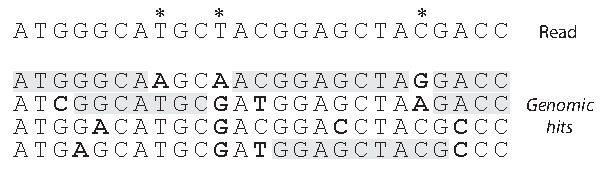
\includegraphics[scale=1]{MEM_example.pdf}
\caption{\textbf{A concrete example of MEM seeding.}
A DNA fragment is sequenced with an imperfect instrument. It comes from
the top genomic location (Truth), but three errors were introduced
(indicated by stars). The sequence of the DNA fragment has three
duplicates at other genomic locations, shown below the target. Mismatches
between the read and the candidate sequence are highlighted in bold. MEM
seeds are indicated by grey boxes.}
\label{fig:MEM_example}
\end{figure}

The MEM seeds are indicated by grey boxes. Technically, they are part of
the read, but they are shown on the genome to highlight the position of
the match. One MEM seed cannot cover a smaller one (otherwise the smaller
would not be a MEM seed), but two consecutive MEM seeds can overlap, as in
the case of the frst two from the left. Note that overlapping MEM seeds
must match distinct sequences of the genome (otherwise neither of them
would be a MEM seed). Consecutive MEM seeds can also be disjoint, as in
the case of the second and the third from the left. In this case, they
must be separated by a nucleotide that is a mismatch against \emph{all}
the duplicates.

Observe that the rightmost MEM seed matches two genomic locations. This
case motivates the following definition, which will play an important role
for the development of the theory.

\begin{definition}
A \emph{strict} MEM seed has a single genomic match.
A \emph{shared} MEM seed has several genomic matches.
\end{definition}

Without surprise, the principle of MEM seeding is to use the genomic
matches of MEM seeds as candidate locations. Importantly, MEM seeds
shorter than a certain threshold $\gamma$ are ignored (in line with the
observation that short matches are uninformative). The parameter $\gamma$
is the tuning knob on the speed/accuracy trade-off. In
Fig.~\ref{fig:MEM_example} for instance, if $\gamma = 7$, there are three
candidate locations (the first, the second and the fourth) and if $\gamma
= 8$ there are only two (the first and the fourth).

Not every MEM seed makes the target a candidate location, so we introduce
the following terms to simplify the discussion.

\begin{definition}
Assume that the thresohld $\gamma$ is fixed. A \emph{good} seed is an
on-target MEM seed of size $\gamma$ or greater. Every other MEM seed is a
\emph{bad} seed. In other words, the true location is in the candidate set
if and only if the read has a good seed.
\end{definition}

Compared to seeds of fixed size, MEM seeds have at least two
counter-intuitive properties. The first is that there are cases where
there is no good seed, even when $\gamma$ is decreased.
Fig.~\ref{fig:full_masking_example} shows such an example. Even though
there is a single sequencing error, the read does not have any MEM seed
matching the target. Lowering $\gamma$ does not change this, so there is
no way to discover the true location (even though it is also the best
location).

\begin{figure}[h]
\centering
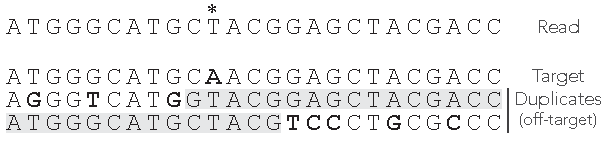
\includegraphics[scale=1]{full_masking_example.pdf}
\caption{\textbf{MEM masking case 1.}
The read, the MEM seeds and the sequences are as in
Fig.~\ref{fig:MEM_example}. The MEM seeds matching the two incorrect
locations at the bottom effectively mask the target, so it cannot
be discovered. MEM masking can occur even when the true location is the
best and when there is a single error on the read.}
\label{fig:full_masking_example}
\end{figure}

The second counter-intuitive property of MEM seeding is that there are
cases where there would be a good seed if the read were shorter.
Fig.~\ref{fig:short_vs_long} shows an example of this case. Again, there
is no on-target MEM seed, but there would be if the read were two
nucleotides shorter on the right side. Indeed, in this case there would be
a shared MEM seed matching the first and the second locations. It would
also be a good seed for $\gamma \leq 12$.


\begin{figure}[h]
\centering
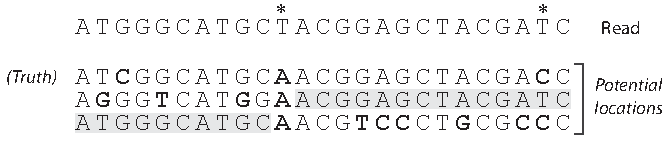
\includegraphics[scale=1]{short_vs_long_example.pdf}
\caption{\textbf{MEM masking case 2.}
The read, the MEM seeds and the sequences are as in
Fig.~\ref{fig:MEM_example}. There is no on-target MEM seed, but there
would be a shared MEM seed if the read were two nucleotides shorter. The
true location has been masked by sequencing the last two nucleotides.}
\label{fig:short_vs_long}
\end{figure}

These examples show that MEM seeds can perform worse than seeds of fixed
size, again raising the question why they seem to give good performance in
practice. The theory developed below will allow us to compute the
probability that a read has no good seed and thus that the true location
is missed. This probability is the key to evaluating and calibrating the
MEM seeding heuristic.

Before going further, we recommend the readers that are not already
familiar with MEM seeding to take a moment to study the examples above.
The complexity of the next sections will go \textit{crescendo} and they
will draw heavily from the concepts and definitions above.


\section{Combinatorial construction of reads}

In this section we represent reads as combinatorial ojects. The
construction has two essential purposes: the first is to give a generative
model of reads that do not have any on-target MEM seed; the second is to
allow us to find the weighted generating function of those reads, which in
turn will allow us to find their probability of occurrence.

\subsection{The MEM alphabet}

The nucleotide sequence of the read is inadequate to know where MEM seeds
are and whether they are on target. For this purpose, we will recode reads
as sequences of letters from the four letter \emph{MEM alphabet}
$\{\downarrow, \uparrow, |, \square\}$.

Each nucleotide is recoded with $\downarrow$, $\uparrow$, or $\square$.
The $\downarrow$ symbol indicates that the nucleotide is a sequencing
error. By definition, it is a mismatch for the target. The $\uparrow$
symbol indicates that the nucleotide is the ``first'' nucleotide of an
on-target MEM seed, which we are about to clarify. All the other
nucleotides are represented by the $\square$ symbol. Finally, the $|$
symbol is appended after the last nucleotide of the read. It is an
obligatory terminator that does not correspond to an actual nucleotide.

To explain the precise meaning of the $\uparrow$ symbol, let us consider
the left end of the read: as we try to extend the first match as much as
possible to the right, the number of hits in the genome decreases. It may
be the case that at some point, there is a single hit and that it is on
target. The very first nucleotid where that happens is called the
\emph{pivot} and is labelled with the symbol $\uparrow$. An on-target MEM
seed has exactly one pivot, so the number of $\uparrow$ symbols is the
number of on-target MEM seeds in the read. Note that $\uparrow$ symbols
marks all on-target MEM seeds, regardless of their size.

Fig.~\ref{fig:sketch_MEM} shows the read of Fig.~\ref{fig:MEM_example} as
encoded with the MEM alphabet. Below the read are the matches between the
read and the potential locations from Fig.~\ref{fig:MEM_example}. A black
square means that the nucleotide is a mismatch for the genomic sequence,
and a white or grey square means that it is a match. Grey squares are used
to highlight MEM seeds, as in Fig.~\ref{fig:MEM_example}.


\begin{figure}[h]
\centering
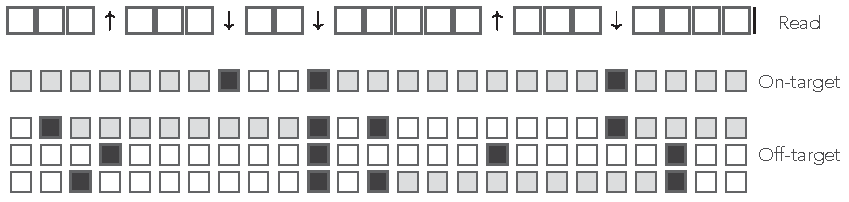
\includegraphics[scale=.85]{sketch_MEM.pdf}
\caption{\textbf{The MEM encoding}.
The read of Fig.~\ref{fig:MEM_example} is recoded with the MEM alphabet.
The mismatches between the read and the potential locations are indicated
with black boxes and the matches with white boxes. The grey boxes are
matches and they indicate the locations of the MEM seeds. The $\downarrow$
symbols coincide exactly with the mismatches between the read and the
target. The $\uparrow$ symbol is always a match for the target and a
mismatch for some off-target location. It indicates the presence of a
strict on-target MEM seed (flanked by the nearest $\downarrow$ symbols or
by the end of the read). Also note the presence of the $|$ terminator at
the end of the read.}
\label{fig:sketch_MEM}
\end{figure}

Observe that the two on-target MEM seeds contain a pivot, but the shared
MEM seed does not. This is always the case. Recall that the pivot
indicates that the true location is the \emph{only} local match, so the
$\uparrow$ symbol cannot appear in on-target MEM seeds when they are
shared.

The MEM alphabet makes it easy to find strict on-target MEM seeds: they
are the longest stretches of symbols containing $\uparrow$ and not
containing $\downarrow$. However, shared on-target MEM seeds do not appear
in this representation.


\subsection{The extended MEM alphabet}

To make shared on-target MEM seeds apparent, we decorate the $\uparrow$
and $\downarrow$ symbols, effectively extending the alphabet. The
$\downarrow$ symbol is replaced by the set of symbols $\downarrow_{/m}$,
where $m$ is the number of duplicates that \emph{match} the erroneous
nucleotide. The $\uparrow$ symbol is replaced by the set of symbols
$\uparrow_{/j}$, where $j-1$ is the number of consecutive $\square$
symbols preceding $\uparrow$.

Note that the numbers decorating the symbols have a very different nature.
In the case of the $\downarrow$ symbol, it is an information about the
number of sequences matching the read; in the case of the $\uparrow$
symbol, it is the position of the pivot relative to the previous
sequencing error (or relative to the beginning of the read).

\begin{figure}[h]
\centering
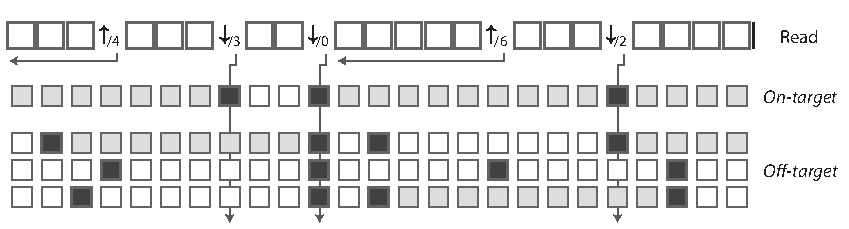
\includegraphics[scale=.85]{sketch_extended.pdf}
\caption{\textbf{The extended MEM encoding}.
The read of Fig.~\ref{fig:sketch_MEM} is represented in the extended MEM
alphabet. The symbols $\uparrow$ and $\downarrow$ are now decorated by
numbers. The arrows departing from those numbers help understand their
meaning. The $\downarrow$ symbol is decorated by the number of locations
that match the nucleotide. The $\uparrow$ symbol is decorated by the
number of consecutive $\square$ symbols before it, plus one.}
\label{fig:sketch_extended}
\end{figure}

Fig.~\ref{fig:sketch_extended} shows the encoding of the read from
Fig.~\ref{fig:sketch_MEM} in the extended MEM alphabet. The arrows bring
the focus on how the numbers decorating the $\uparrow$ and $\downarrow$
symbols are computed. For instance, the $\downarrow_{/0}$ symbol indicates
that the nucleotide is an error (this is the meaning of the $\downarrow$
symbol), and that it matches no other location (this is meaning of $/0)$.
In other words, it is a mismatch against every potential location.

In this new encoding, shared on-target MEM seeds are stretches of
$\square$ symbols flanked either by $\downarrow_{/0}$, or by $|$, or by
the left end of the read. Indeed, such a stretch is a MEM seed because it
matches at least one sequence (the target) and it cannot be extended
(because the end of the read is reached or because there is no match in
the genome). Also, it cannot be a strict on-target MEM seed because it
does not contain the $\uparrow$ symbol, so it must be a shared on-target
MEM seed.

The reason for introducing more than just the $\downarrow_{/0}$ symbol is
not immediately clear. For the combinatorial construction to be useful, we
need not only to identify on-target MEM seeds, but also to compute the
probabilities of the reads of each type. This is precisely the role of the
extended alphabet, as we will see in section~\ref{sec:transfer_mat}.

\subsection{Reads as extended MEM segments}

The final twist in the combinatorial construction is to consider reads not
as sequences of symbols, but as sequences of \emph{segments}. The purpose
here is merely to express that some on-target MEM seeds are good
(\textit{i.e.}, their size is $\gamma$ or greater) and some are not.


\begin{definition}
\label{def:segment}
A segment is a maximal sequence of $\square$ symbols flanked on the right
side by one of the symbols $\uparrow_{/j}$, $\downarrow_{/m}$, or $|$. The
one and only segment flanked by $|$ is called the tail. It is the only
segment that can have size 0.
\end{definition}


In line with definition~\ref{def:segment}, the symbols $\uparrow_{/j}$,
$\downarrow_{/m}$ and $|$ are referrred to as \emph{terminators}.
Fig.~\ref{fig:sketch_segment} shows the segment representation of the read
from Fig.~\ref{fig:sketch_extended}. The numbers below indicate the size
of each segment.

\begin{figure}[h]
\centering
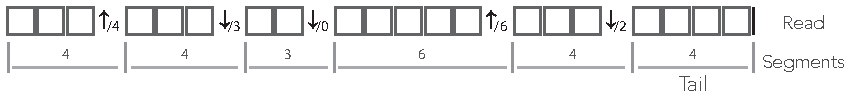
\includegraphics[scale=.85]{sketch_segments.pdf}
\caption{\textbf{The extended MEM segment encoding}.
The read from Fig.~\ref{fig:sketch_segment} is represented as a sequence
of segments. Each segment is terminated by either $\uparrow_{/j}$, or
$\downarrow_{/m}$ or $|$. The rightmost fragment is the tail. The numbers
below indicate the size of each segment in nucleotides.}
\label{fig:sketch_segment}
\end{figure}

Shared on-target MEM seeds at the tail of the read are segments but all
other on-target MEM seeds are not. Shared MEM seeds cannot contain the
terminator $\downarrow_{/0}$ because it is a mismatch against the target.
Strict on-target MEM seeds are split over at least two segments: one
terminated by $\uparrow_{/j}$ and one right of it terminated by either
$\downarrow_{/m}$ or $|$.


\section{Symbolic and analytic representations}

We now turn to the question of translating the extended MEM segment
representation to a construction of reads without good seeds
(\textit{i.e.}, without on-target MEM seeds of size $\gamma$ or greater).
For this, we use tools borrowed from analytic combinatorics. We give the
minimum amount of background that is necessary to expose the theory. A
more detailed account of the strategy to compute seeding probabilities
with analytic combinatorics has been published
elsewhere\cite{filion2017analytic,filion2018analytic}. We refer the
readers interested in learning more about analytic combinatorics to the
textbooks\cite{flajolet2009analytic,sedgewick2013introduction}.

\subsection{Weighted generating functions}

Let $\mathcal{A}$ be a set of combinatorial objects with a size $k \in
\mathbb{N}$ and a probability of occurrence. Denoting $a_k$ the total
probability of objects of size $k$, the function defined as $A(z) =
\sum_{k\geq0} a_kz^k$ is called the \emph{weighted generating
function} of the combinatorial objects.

In our case, we are interested in the weighted generating function of
reads without good seeds, so the coefficient $a_k$ is the probability
that a read of size $k$ has no good seed. As $k$ becomes larger,
it becomes more difficult to evaluate $a_k$, but the representation
developed above will allow us to do this.


\subsection{The symbolic method}

The symbolic method is a strategy belonging to the general \emph{analytic
combinatorics} framework. The idea is to combine simple combinatorial
objects into more complex objects. Each combinatorial operation on the
objects corresponds to a mathematical operation on their weighted
generating functions. One can thus obtain the weighted generating function
of complex objects, and from there extract their probability of
occurrence.

The combinatorial construction of reads using the extended MEM alphabet
gives us a method to express their weighted generating function from the
simpler generating function of segments. More specifically, we can
describe complex sequences of segments through a so-called \emph{transfer
matrix} $M(z)$ that specifies which pairs of consecutive segments are
allowed and which are forbidden in the reads of interest.

The segment types are identified by their terminators arranged in a
predefined oder. The entry of $M(z)$ at coordinates $(i,j)$ is the
weighted generating function of segments with the $j$-th terminator that
can be inserted immediately after segments with the $i$-th terminator. The
entries of the matrix $M(z) + M(z)^2 + \ldots = M(z) \cdot (I-M(z))^{-1}$
are the weighted generating functions of the reads of all sizes using all
the allowed combinations of segments.

The entry of interest from $M(z)$ is the one that corresponds to the
terminators $\downarrow_{/0}$ and $|$ because it represents the reads of
any size whose first segment can be inserted after $\downarrow_{/0}$, and
whose last segment is terminated by $|$. Indeed, the $|$ terminator marks
the end of the read, so it must be the final symbol of every valid read.
As for the first segment, observe that all the segments that can follow
the $\downarrow_{/0}$ symbol are exactly those that can be at the frst
postion of the read\footnote{One could have introduced a special start
symbol. It is equivalent to an invisible $\downarrow_{/0}$ prepending
the reads.}.

In summary, the transfer matrix $M(z)$ contains the weighted generating
function of interest. Our next task is thus to specify $M(z)$.



\section{The transfer matrix}
\label{sec:transfer_mat}

\subsection{Hard and soft masking}

For each potential location including the target, we define the
\emph{match streak} at a given nucleotide as the number of nucleotides
since the last mismatch on the left. For instance, in
Fig.~\ref{fig:MEM_example}, the match streak of the target at the ninth
nucleotide is $1$ while for the second potential location, it is $7$.

\begin{definition}
At a given position of the read, an off-target location is a \emph{hard
mask} if its success streak is strictly longer than the match streak of
the target. An off-target location is a \emph{soft mask} if its has the
same match streak as the target.
\end{definition}

For instance, the second location in the example above is a hard mask at
the ninth nucleotide. On Fig.~\ref{fig:MEM_example}, one can further check
that all the off-target locations are soft masks at the second nucleotide
and that the second location is a soft mask at the last nucleotide of the
read.

A nucleotide with a hard mask cannot be part of an on-target MEM seed. A
nucleotide without mask belongs to a strict on-target MEM seed. A
nucleotide with a soft mask may belong to a strict on-target MEM seed, to
a shared on-target MEM seed, or may not belong to any MEM. This case is
the most intricate and it will be teased apart below.

The extended MEM alphabet is nothing more than a way to keep track of the
hard and soft masks. For instance, a pivot (associated with the symbols
$\uparrow_{/j}$) is a nucleotide where the number of masks becomes 0.
Denoting the number of off-target locations by $N$, the symbol
$\downarrow_{/m}$ indicates that there are $m$ hard masks and $N-m$ soft
masks.


\subsection{Error model and divergence of the duplicates}

We assume that the target sequence has $N$ duplicates. We further assume
that duplication was instantaenous and that all $N+1$ sequences diverge
independently from each other at a constant rate. In other words, we
ignore the complications due to the genealogy of the duplication events
and we simply assume that at each position, any given duplicate is
identical to the target with probability $1-\mu$. If it is not, we
assume that the duplicate has any of the remaining three nucleotides with
equal probability (\textit{i.e.} each is found with probability $\mu/3$).

We also assume that the sequencing instrument has a constant substitution
rate $p$, and that insertions and deletions never occur. In case of a
substitution, we again assume that the remaining three nucleotides are
equally likely.

On a read error the target is never identical to the read (because we
assume that the target is the true sequence), and a duplicate is identical
to the read with probability $mu/3$ (the probability that the duplicate is
different from the target, times the probability that the nucleotide is
the same as the error). On a correct nucleotide, the target is always
identical to the read, and a dupicate is identical with probability
$1-\mu$ (the probablity that the duplicate is identical to the target).

With these assumptions, we are now ready to describe the entries of the
transfer matrix $M(z)$, which we do in order of increasing difficulty.


\subsection{Segments following $\uparrow_{/j}$}

A $\uparrow_{/j}$ symbol marks a pivot and the absence of masks. The
segment is thus the beginning of an on-target MEM of size at least $j$.
The MEM will extend until the next sequencing error, or until the end of
the read, so the number of $\square$ symbols in the next segment must be
at most $\gamma-j-1$ and it must be terminated by a $\downarrow$ symbol or
by the tail terminator $|$.

In this case, the matches between the read and the duplicates are
irrelevant until the terminator. The weighted genearting function of each
$\square$ symbol is simply $qz$ ($q$ is the probability that the
nucleotide is not an error and $z$ marks objects of size $1$).

\begin{definition}
The probability that a symbol is $\downarrow_{/m}$ given that the
nucleotide is a read error is
\begin{equation}
\label{eq:omega}
\omega_m = {N \choose m} \big(1 - \mu/3\big)^{N-m} \big(\mu/3\big)^m.
\end{equation}
\end{definition}

The weighted generating function of the $\downarrow_{/m}$ terminator is
thus $\omega_m pz$ (the probability of the $\downarrow_{/m}$ is $\omega_m
p$ and $z$ marks objects of size $1$).

The entries of the transfer matrix that correspond to transitions from
$\uparrow_{/j}$ to other segments are now easy to find. The weighted
generating function of the segments terminated by $\downarrow_{/m}$
following a segment terminated by $\uparrow_{/j}$ is
\begin{equation}
\label{eq:D}
D_{j,m}(z) = \omega_m pz \sum_{i=0}^{\gamma-j-1} (qz)^i.
\end{equation}

And the weighted generating function of the tail segments following
segments terminated by $\uparrow_{/j}$ is
\begin{equation}
\label{eq:E}
E_j(z) = \sum_{i=0}^{\gamma-j-1} (qz)^i.
\end{equation}


\subsection{Segments following $\downarrow_{/m}$}

At a $\downarrow_{/m}$ symbol, there are $m$ hard masks and $N-m$ soft
masks. If all the masks disappear before the first read error, the next
terminator will be a $\uparrow$ symbol, otherwise it will be a
$\downarrow$ symbol.

\subsubsection*{Case 1: the terminator is $\uparrow_{/i}$}

\begin{definition}
The probability that a given duplicate sequence contains a mismatch in a
sequence of $i$ error-free nucleotides is
\begin{equation}
\label{eq:xi}
\xi_i = 1-(1-\mu)^i.
\end{equation}
\end{definition}

With this notation, the probability that at least one mask survives a
sequence of $i$ error-free nucleotides is thus $1-\xi_i^N$, and the
probability that there remains a mask at the $i-1$-th but not at the 
$i$-th error-free nucleotide is $\xi_i^N - \xi_{i-1}^N$. From this we
conclude that the weighted generating function of the segments terminated
by $\uparrow_{/i}$ following a segment terminated by $\downarrow_{/m}$ is
\begin{equation}
\label{eq:B}
B_i(z) = \Big( \xi_i^N-\xi_{i-1}^N \Big) (qz)^i.
\end{equation}

In the equation above, $q^i$ is the probability that there is no
sequencing error in $i$ nucleotides and $z^i$ marks objects of size $i$.
As mentioned above, $i < \gamma$ for reads without on-target MEM seed.
Also note that this expression is the same for all $\downarrow$ symbols;
it does not depend on $m$.

\subsubsection*{Case 2a: the terminator $|$ comes before the $\gamma$-th
nucleotide}

In this case there can be no on-target MEM seed. We must just enforce the
condition that at least one of the $N$ masks survives until the end of the
segment in order to exclude the $\uparrow$ symbol. The weighted generating
function is
\begin{equation*}
\sum_{i=0}^{\gamma-1} \Big(1 - \xi_i^N \Big) (qz)^i.
\end{equation*}

\subsubsection*{Case 2b: the terminator $|$ comes after the $\gamma$-th
nucleotide}

In this case, the soft masks are irrelevant. Even if they survive until
the end of the segment, there will be a shared on-target MEM seed. So we
must enforce the condition that at least one hard mask survives until the
end of the segment (which is impossible if $m = 0$).
\begin{equation*}
\sum_{i=\gamma}^\infty \Big(1 - \xi_i^m \Big) (qz)^i.
\end{equation*}

The transition from $\downarrow_{/m}$ to $|$ is
\begin{equation}
\label{eq:C}
C_m(z) =
\sum_{i=0}^{\gamma-1} \Big(1 - \xi_i^N \Big) (qz)^i +
  \sum_{i=\gamma}^\infty \Big(1 - \xi_i^m \Big) (qz)^i.
\end{equation}

\subsubsection*{Case 3a: the terminator $\downarrow_{/n}$ comes before the
$\gamma$-th nucleotide}

As above, there can be no on-target MEM seed and we must just exclude the
$\uparrow$ terminator. The weighted generating function is
\begin{equation}
\omega_n pz \sum_{i=0}^{\gamma-1} \Big(1 - \xi_i^N \Big) (qz)^i.
\end{equation}

\subsubsection*{Case 3a: the terminator $\downarrow_{/n}$ comes after the
$\gamma$-th nucleotide}

This case is by far the most convoluted. Since the segment contains at
least $\gamma$ error-free nucleotides, we must take care that it does not
generate an on-target MEM seed. This will be the case if any of the two
following conditions is validated: $i)$ at least one hard mask covers all
the error-free nucleotides, or $ii)$ none of the hard masks does but at
least one soft mask covers the whole segment (including the terminator).

The two conditions are mutually exclusive by construction. They are
graphically represented in the diagram below. The left panel corresponds
to case $i)$ and the panel to case $ii)$. The top row represents the
target, and the bottom rows represent duplicates (using the same
symbols as in Fig.~\ref{fig:sketch_MEM}).
\begin{inset}
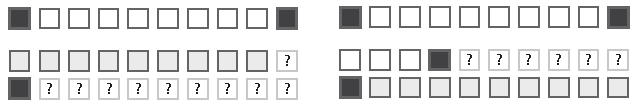
\includegraphics{masks.pdf}
\end{inset}

Whenever a hard mask (here the first duplicate) covers the nucleotides
as shown in the left panel, there can be no on-target MEM seed,
irrespective of the value of $\gamma$. The positions marked with a
question mark are irrelevant, they cannot change the fact that there is no
on-target MEM seed. If the hard masks are interrupted, as in the right
panel, then it depends on the soft masks. If a soft mask covers the whole
segment, then there can be no on-target MEM seed, irrespective of the
value of $\gamma$.

Condition $i)$ has probability $\big(1 - \xi_i^m \big)$ and the
weighted generating function is thus
\begin{equation*}
\omega_n pz \sum_{i=\gamma}^\infty \Big(1 - \xi_i^m \Big) (qz)^i.
\end{equation*}

For condition $ii)$, we will need to introduce some new notations.
\begin{definition}
The probability that a given duplicate sequence contains a mismatch in a
sequence of $i$ error-free nucleotides followed by an error is
\begin{equation}
\label{eq:eta}
\eta_i = 1-(1-\mu)^i\mu/3.
\end{equation}
\end{definition}

The probability of condition $ii)$ is
\begin{equation*}
\xi_i^m \Big(1 - \eta_i^{N-m} \Big),
\end{equation*}
but we need to break up this term among the terminators $\downarrow_{/n}$,
($0 \leq n \leq N$). For this, we decompose the sum on the number of soft
masks that run to the end of the segment, including the terminator. The
probability that there are $r \geq 1$ such soft masks is
\begin{equation*}
{N-m \choose r} (1 - \eta_i)^r \eta_i^{N-m-r}.
\end{equation*}

Each of them matches the nucleotide at the end of the segment, so the
total number of matches is $r$ plus the number of sequences, among the
remaining $N-m-r$ soft masks and $m$ hard masks, that also match the
last nucleotide.

Let us start with the $N-m-r$ that failed somewhere in the segment. The
conditional probability that they match the last nucleotide given that
they fail somewhere in the segment is $\mu/3 \cdot \xi_i / \eta_i$. The
conditional probability that they do not match is $(1-\mu/3) / \eta_i$.
For the $m$ hard masks, the probability that they match the last
nucleotide given that they sail somewhere in the segment is simply
$\mu/3$, and the probability that they do not is $1-\mu/3$.

The probability that those $N-r$ duplicates contribute $n-r$ matches is
\begin{equation*}
\frac{(\mu/3)^{n-r}(1-\mu/3)^{N-n}}{\eta_i^{N-m-r}}
\psi_{i,m,n,r}\text{, where \;}
\psi_{i,m,n,r} = \sum_{q \geq 0}{m \choose q}{N-m-r \choose n-r-q}
\xi_i^{n-r-q}.
\end{equation*}


The probability that in
total $n$ sequences match the terminator is
\begin{eqnarray*}
&\;& \sum_{r\geq1} {N-m \choose r}
(1 - \eta_i)^r (\mu/3)^{n-r} (1-\mu/3)^{N-n} \psi_{i,m,n,r} \\
&=& (\mu/3)^n(1-\mu/3)^{N-n} \sum_{r\geq1} {N-m \choose r}
  (1 - \mu)^{ri} \psi_{i,m,n,r} \\
&=& \omega_n \cdot \zeta_{i,m,n},
\end{eqnarray*}
where
\begin{equation}
\label{eq:zeta}
\zeta_{i,m,n} = \sum_{r\geq1} {N-m \choose r}
(1-\mu)^{ri} \psi_{i,m,n,r} \bigg/ {N \choose n}.
\end{equation}


The weighted generating function we are looking for is thus
\begin{equation}
\label{eq:A}
A_{m,n} =
\omega_n pz \sum_{i=0}^{\gamma-1} \Big(1 - \xi_i^N \Big) (qz)^i + \omega_n
pz \sum_{i=\gamma}^\infty \Big(1 - \xi_i^m \cdot
(1- \zeta_{i,m,n}) \Big) (qz)^i.
\end{equation}

\subsection{The expression of the transfer matrix}

The final expression for the transfer matrix $M(z)$ is
\begin{equation*}
\begin{blockarray}{cccccccc}
   & \dn{0} & \ldots & \dn{N} & \up{1} & \ldots & \up{\gamma-1} & \nd \\
\begin{block}{c[ccccccc]}
\dn{0} & A_{0,0}(z) & \ldots & A_{0,N}(z) & B_1(z) & \ldots &
    B_{\gamma-1}(z) & C_0(z) \\
\vdots & \vdots & \ddots & \vdots & \vdots & \ddots &
    \vdots & \vdots \\
\dn{N} & A_{N,0}(z) & \ldots & A_{N,N}(z) & B_1(z) & \ldots &
    B_{\gamma-1}(z) & C_N(z) \\
\up{1} & D_{1,0}(z) & \ldots & D_{1,N}(z) & 0 & \ldots & 0 & E_1(z) \\
\vdots & \vdots & \ddots & \vdots & \vdots & \ddots &
    \vdots & \vdots \\
\up{\gamma-1} & D_{\gamma-1,0}(z) & \ldots & D_{\gamma-1,N}(z) & 0 &
  \ldots & 0 & E_{\gamma-1}(z) \\
\nd & 0 & \ldots & 0 & 0 & \ldots & 0 & 0 \\
\end{block}
\end{blockarray}
\end{equation*}
where
\begin{gather}
\tag{\ref{eq:A}}
A_{m,n} =
\omega_n pz \sum_{i=0}^{\gamma-1} \Big(1 - \xi_i^N \Big) (qz)^i + \omega_n
pz \sum_{i=\gamma}^\infty \Big(1 - \xi_i^m \cdot
(1- \zeta_{i,m,n}) \Big) (qz)^i \\
\tag{\ref{eq:B}}
B_i(z) = \Big( \xi_i^N-\xi_{i-1}^N \Big) (qz)^i \\
\tag{\ref{eq:C}}
C_m(z) =
\sum_{i=0}^{\gamma-1} \Big(1 - \xi_i^N \Big) (qz)^i +
  \sum_{i=\gamma}^\infty \Big(1 - \xi_i^m \Big) (qz)^i \\
\tag{\ref{eq:D}}
D_{j,m}(z) = \omega_m pz \sum_{i=0}^{\gamma-j-1} (qz)^i \\
\tag{\ref{eq:E}}
E_j(z) = \sum_{i=0}^{\gamma-j-1} (qz)^i
\end{gather}
and where
\begin{gather}
\tag{\ref{eq:omega}}
\omega_m = {N \choose m} \big(1 - \mu/3\big)^{N-m} \big(\mu/3\big)^m \\
\tag{\ref{eq:xi}}
\xi_i = 1-(1-\mu)^i \\
\tag{\ref{eq:eta}}
\eta_i = 1-(1-\mu)^i\mu/3 \\
\tag{\ref{eq:zeta}}
\zeta_{i,m,n} = \sum_{r\geq1} {N-m \choose r}
(1-\mu)^{ri} \psi_{i,m,n,r} \bigg/ {N \choose n} \\
\notag
\psi_{i,m,n,r} = \sum_{q \geq 0}{m \choose q}{N-m-r \choose n-r-q}
\xi_i^{n-r-q}.
\end{gather}


\section{Computing the probabilities}

\subsection{Coefficient extraction}

The purpose of constructing the weighted generating function $F(z) = a_0 +
a_1z + a_2z^2 + \ldots$ is to extract the coefficient $a_k$, which
represents the probability that a read of size $k$ does not contain an
on-target MEM seed. $F(z)$ is the entry at coordinates $(1,N+\gamma+1)$ of
the matrix $M(z) \cdot (I-M(z))^{-1}$. The expression of $M(z)$ is in
general too complex to compute this function directly. Instead, we return
to the expression $M(z) \cdot (I-M(z))^{-1} = M(z) + M(z)^2 + \ldots$ and
observe that the terms $M(z)^{k+2}, M(z)^{k+3}, \ldots$ have no influence
on the coefficients $a_0, a_1, \ldots, a_k$.

Indeed, a read of size $k$ has at most $k+1$ segments. Since the entries
of $M(z)^k$ are the weighted generating functions of reads with exactly
$k$ segments, $a_k$ cannot depend on $M(z)^{k+2}, M(z)^{k+3}$. More
formally, we can prove by induction that all the entries of $M(z)^k$ are
divisible by $z^{k-1}$, showing that the contribution of $M(z)^{k+2} +
M(z)^{k+3} + \ldots$ to $a_0 + a_1z + \ldots +a_kz^k$ is $0$.

So we can extract the coefficients of $F(z)$ up to order $k$ by computing
the matrix $M(z) + M(z)^2 + \ldots + M(z)^{k+1}$, and compute the first
terms of the Taylor expansion of the entry at coordinates
$(1,N+\gamma+1)$.

But we can do better than that. If we are only interested in the
coefficients of order up to $k$, we can replace the infinite power series
of the terms $A_{m,n}(z)$ and $C_m(z)$ by their truncated versions where
we keep only the terms of order up to $k$. Likewise, we perform all
algebraic operation on truncated polynomials of order $k$, \textit{i.e.}
we discard at every stage the coefficients of order greater than $k$. With
this approach, the entry of the matrix $M(z) + M(z)^2 + \ldots +
M(z)^{k+1}$ at coordinates $(1,N+\gamma+1)$ is a truncated polynomial that
directly provides the coefficients of interest.

But we can do better than that. A read with $k$ segments contains at least
$(k-1)/2$ errors. Indeed, two segments terminated by $\uparrow$ cannot
follow each other, so at least (approximately) half of the segments must
be terminated by $\downarrow$, which means that the segment contains a
read error. Since read errors typically have a small probability of
occurrence, all the coefficients of $M(z)^k$ rapidly converge to $0$ and
become negligible as $k$ increases. So instead of computing $M(z) + M(z)^2
+ \ldots + M(z)^{k+1}$, we can interrupt the summation after a certain
power of $M(z)$ because the terms are negligible.

This approach makes it feasible to compute the probability that a read of
size $k$ has no on-target MEM seed when the matrix $M(z)$ is small, but
recall that $M(z)$ has dimension $N+\gamma+1$. Some sequences can have
million of duplicates in mammalian genomes (\textit{i.e.} $N > 10^6$),
which makes the computations with this method unfeasible. Clearly, another
method is needed.


\subsection{Monte Carlo sampling}

The symbolic representation of reads in the extended MEM alphabet can also
be used as a basis for an efficient method to sample reads. Instead of
generating the nucleotides of each sequence one by one and comparing them
to the read, one can generate segments of the extended MEM alphabet. As
argued above, a read contains few segments when the error rate is small.
Since this property does not depend on the value of $N$, we can obtain a
fast Monte Carlo method to sample millions of reads and count the
proportion that contain an on-target MEM seed.

The principle is to first sample the position of the next read error, and
then sample the number of masks that survive until this position. If none
of the does, the read contains an on-target MEM seed, provided the next
read error is at a distance greater than $\gamma$. Otherwise, the process
is repeated for the next segment until an on-target MEM seed is generated,
or until the read has size $k$ or greater (and is then truncated).

The method is summarized by the algorithm below (FIX THE ALGORITHM).

\begin{algorithm}[H]
\SetAlgoLined
\KwResult {Sample a read, return 1 if it contains an on-target MEM seed,
  otherwise return 0.}
  $read.size \leftarrow 0$\;
  $m \leftarrow 0$ \Comment*[r]{Current number of hard masks.}
  \While {$read.size < k$}{
    $i \leftarrow geom(p)$ \Comment*[r]{Position of next error.}
    \eIf {$read.size + i > k$}{
      $\lambda \leftarrow k - read.size$ \Comment*[r]{Size of the tail.}
      \eIf{$\lambda < \gamma$} {
        return 0\; }{
        $h \leftarrow binom(m,(1-\mu)^\lambda)$
            \Comment*[r]{Surviving hard masks.}
        return 1 if $h = 0$, otherwise return 0\; }
    }
    {
      $h \leftarrow binom(m,(1-\mu)^i)$
          \Comment*[r]{Surviving hard masks.}
      $s \leftarrow binom(N-m,(1-\mu)^i \mu/3)$
          \Comment*[r]{Surviving soft masks.}
      \eIf {$ i \geq \gamma$ and $h = 0$ and $s = 0$}{
        return 1\;}{
        $m \leftarrow s + binom(N-s, \mu/3)$\;
        $read.size \leftarrow read.size + i$\;}
    }
 }
\end{algorithm}

\section{Estimating the parameters}

Let us assume that we have a sequence of length $L$ that has $N$
duplicates in the genome. Let us further assume that the instrument has a
uniform error rate of $p$, and that at each nucleotide, duplicates are
different from the original sequence with probability $\mu$. What are the
values of $p$ and $\mu$ that maximize the probability that the read is
different from the original, but identical to a duplicate?

If the read has no error, this cannot happen. If we consider the reads
with one error, the probability that this happens is
\begin{equation}
Q(p,\mu) = L \cdot p \cdot (1-p)^{L-1}
\cdot \Big( 1- (1-(1-\mu)^{L-1} \mu/3)^N \Big).
\end{equation}

Observe that for every value of $p$, $\mu = 1/L$ maximizes $Q(p,\mu)$. So
in this simple proble, there exists a ``worst'' value of $\mu$, that
maximizes the probability of making a mistake irrespective of the
precision of the sequencing instrument and of the number of duplicates.

The MEM seeding heuristic is more complex than the toy problem above, but
we still get the intuition that values of $\mu$ close to $1/L$ are the
most problematic, where $L$ is the typical size of MEM seeds.

Using the above methods to compute MEM seeding probabilities, we can test
this claim with typical values of the parameters. For the human genome,
seeds of length $\approx 20$ are the norm...

\section{Using the information of the backward search}

Assume that the sequence to map has $N$ additional duplicates, all with a
uniform divergence equal to $\mu$. We can use the number of hits
obtained in the backard search to estimate $N$ and $\mu$.

At every stage of the backward search, we obtain the number of sequences
in the reference genome that match the end of the query. Ignoring
sequencing errors and focusing only on the $N$ duplicates, the probability
that the count of duplicates goes from $N_i$ to $N_{i+1}$ at each step of
the search is given by

\begin{equation*}
P(N_{i+1}|N_i) = {N_i \choose N_{i+1}}
\mu^{N_i-N_{i+1}}(1-\mu)^{N_{i+1}}.
\end{equation*}

The probability of the sequence $(N_1, N_2, \ldots,
N_m)$ starting from $N_0$ is

\begin{equation*}
P(N_1, \ldots, N_m|N_0) = 
{N_0 \choose N_1 } \ldots {N_{m-1} \choose N_m }
\mu^{N_0-N_m}(1-\mu)^{N_1+\ldots+N_m}.
\end{equation*}

We can now use the maximum likelihood approach to find the value of
$\mu$ that maximizes this expression. Taking the logarithm and
differentiating with respect to $\mu$ we find

\begin{gather*}
\frac{N_0-N_m}{\mu}-\frac{N_1+\ldots+N_m}{1-\mu} = 0
\text{, which implies} \\
\mu = \frac{N_0-N_m}{N_0+\ldots+N_{m-1}}.
\end{gather*}

We also observe that by defining the loss at each step $\Delta_i = N_{i-1}
- N_i$, the distribution of $(\Delta_1, \ldots, \Delta_m, N_m)$ given
$N_0$ is multinomial with parameters $\big(\mu, \mu(1-\mu),
\ldots, \mu(1-\mu)^{m-1}, (1-\mu)^m\big)$. More specifically, the
probability of observing the sequence $(\Delta_1, \ldots, \Delta_m, N_m)$
given $N_0$ is

\begin{align*}
{N_0 \choose \Delta_1, \ldots, \Delta_m, N_m}
\mu^{\Delta_1}\big(\mu(1-\mu)\big)^{\Delta_2}
\ldots \big(\mu(1-\mu)^{m-1}\big)^{\Delta_m}(1-\mu)^{mN_m}.
\end{align*}

Now, if $N_0, N_1, \ldots, N_{n-1}$ are missing, we can compute the
probability of observing $(\Delta_{n+1}, \ldots, \Delta_m, N_m)$ from the
marginal distribution as

\begin{align*}
\begin{split}
{N_0 \choose N_0-N_n, \Delta_{n+1}, \ldots, \Delta_m, N_m}
\big(1-(1-\mu)^n\big)^{N_0-N_n}
\big(\mu(1-\mu)^n\big)^{\Delta_{n+1}} \times
\ldots \\
\ldots \times
\big(\mu(1-\mu)^{m-1}\big)^{\Delta_m}(1-\mu)^{mN_m}.
\end{split}
\end{align*}

This expression depends on $N_0$, which can be considered a parameter of
the distribution. To estimate it, we take the logarithm of the probability
and differentiate with respect to $N_0$. We obtain the two following
equations

\begin{gather*}
\Psi(N_0+1)-\Psi(N_0-N_n+1) + \log\big( 1-(1-\mu)^n \big) = 0 \\
\frac{N_n-N_m}{\mu}
-\frac{nN_n + N_{n+1}+\ldots+N_m}{1-\mu} +
(N_0-N_n)\frac{n(1-\mu)^{n-1}}{1-(1-\mu)^n} = 0.
\end{gather*}

In the expression above, $\Psi(\cdot)$ is the digamma function, defined as
the derivative of $\log \Gamma(\cdot)$. We observe that the second
equation gives an expression of $N_0$ as a function of $\mu$, namely

\begin{equation*}
N_0 = N_n +
\left(\frac{nN_n+N_{n+1}+\ldots+N_m}{1-\mu}-
\frac{N_n-N_m}{\mu} \right)
\frac{1-(1-\mu)^n}{n(1-\mu)^{n-1}}.
\end{equation*}

We can substitute this expression in the first equation, obtaining an
equation depending on $\mu$ only, which can be solved numerically by
the Newton-Raphson method.

\section{Conclusion}

This is awesome.

\section*{Acknowledgements}

We acknowledge the financial support of the Spanish Ministry of Economy
and Competitiveness (‘Centro de Excelencia Severo Ochoa 2013-2017’, Plan
Nacional BFU2012-37168), of the CERCA Programme~/~Generalitat de
Catalunya, and of the European Research Council (Synergy Grant 609989).


%---------------------------------------------------------------
%---------------------------------------------------------------

\bibliography{references,pubmed}
\bibliographystyle{plain}

%----------------------------------------------------------------

\end{document}

%gs -dNoOutputFonts -sDEVICE=pdfwrite -o out.pdf latex.pdf 
